%---------------------------------

The CPH algorithm is based on a recursive relation  and illustrated by an example in Figure~\ref{fig:SS2}. Figure~\ref{fig:SS2}(a) presents a set of three devices with different operation states. Each state consumes a stable power with a corresponding probability. Assuming at time instant $t$, the aggregate power consumption $x$ is equal to 150~W. With the standard deviation $\epsilon$ of 5~W, the total power demand of any set of operating devices cannot exceed the bound $R=x +\epsilon = 155$~W. Figure~\ref{fig:SS2}(b) shows how the CPH algorithm operates. In the first step, each device is represented as a set of \textit{tuples}, each corresponding to a state. For example, device $D_1$ comprises three tuples: $(0, 23.03,173.03)$, $(50,2.23,102.23)$, $(150,23.03,23.03)$. The first element $d_1$ of each tuple represents the power demand, the second one $d_2$ contains the product of the operating probability in log-linear form and the regularization parameter $\lambda$, equal to 10 in this example, and the third one $d_3$ is calculated from two first elements $d_1$ and $d_2$ as follows:
\begin{eqnarray}
d_1 &=& w\\
d_2 &=& -\lambda \times \log{p}\\
d_3 &=& \left|x-d_1\right|+d_2. \label{eqCPH1}
\end{eqnarray}
\begin{figure}[h]
%\centering
\begin{minipage}[b]{1\linewidth}
  \centering
  \centerline{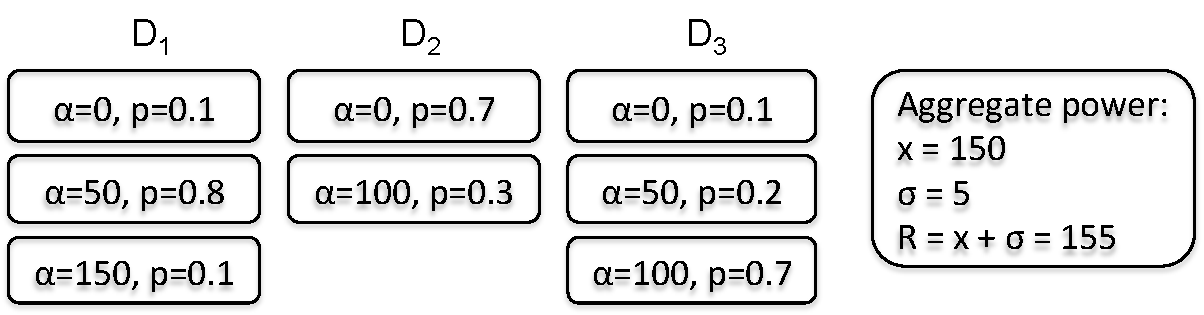
\includegraphics[width=0.8\textwidth]{./chapters/chapter4/images/cph1}}
%  \vspace{2.0cm}
  \centerline{(a)}\medskip
\end{minipage}
\begin{minipage}[b]{1\linewidth}
  \centering
  \centerline{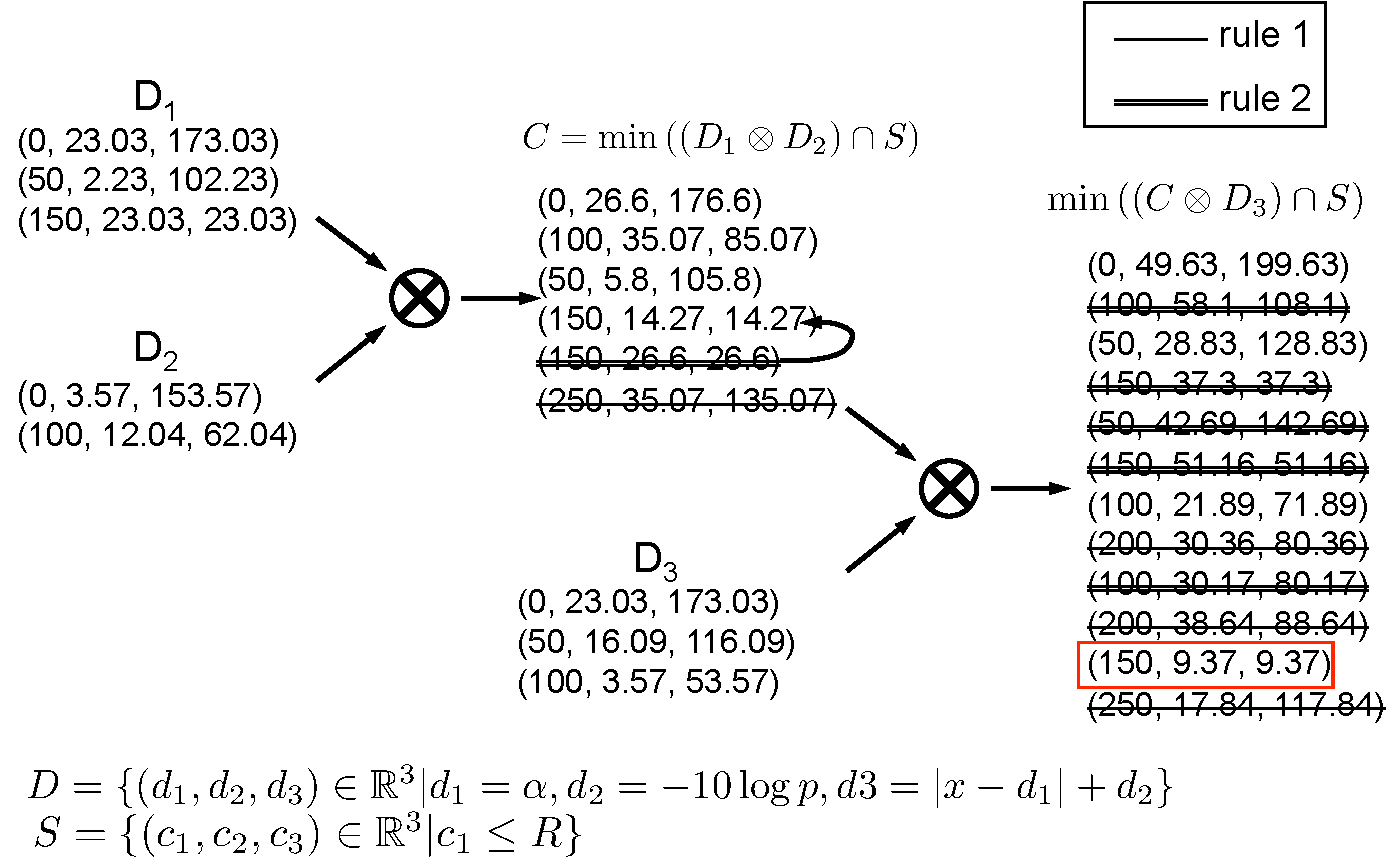
\includegraphics[width=0.9\textwidth]{./chapters/chapter4/images/cph2}}
%  \vspace{2.0cm}
  \centerline{(b)}\medskip
\end{minipage}
%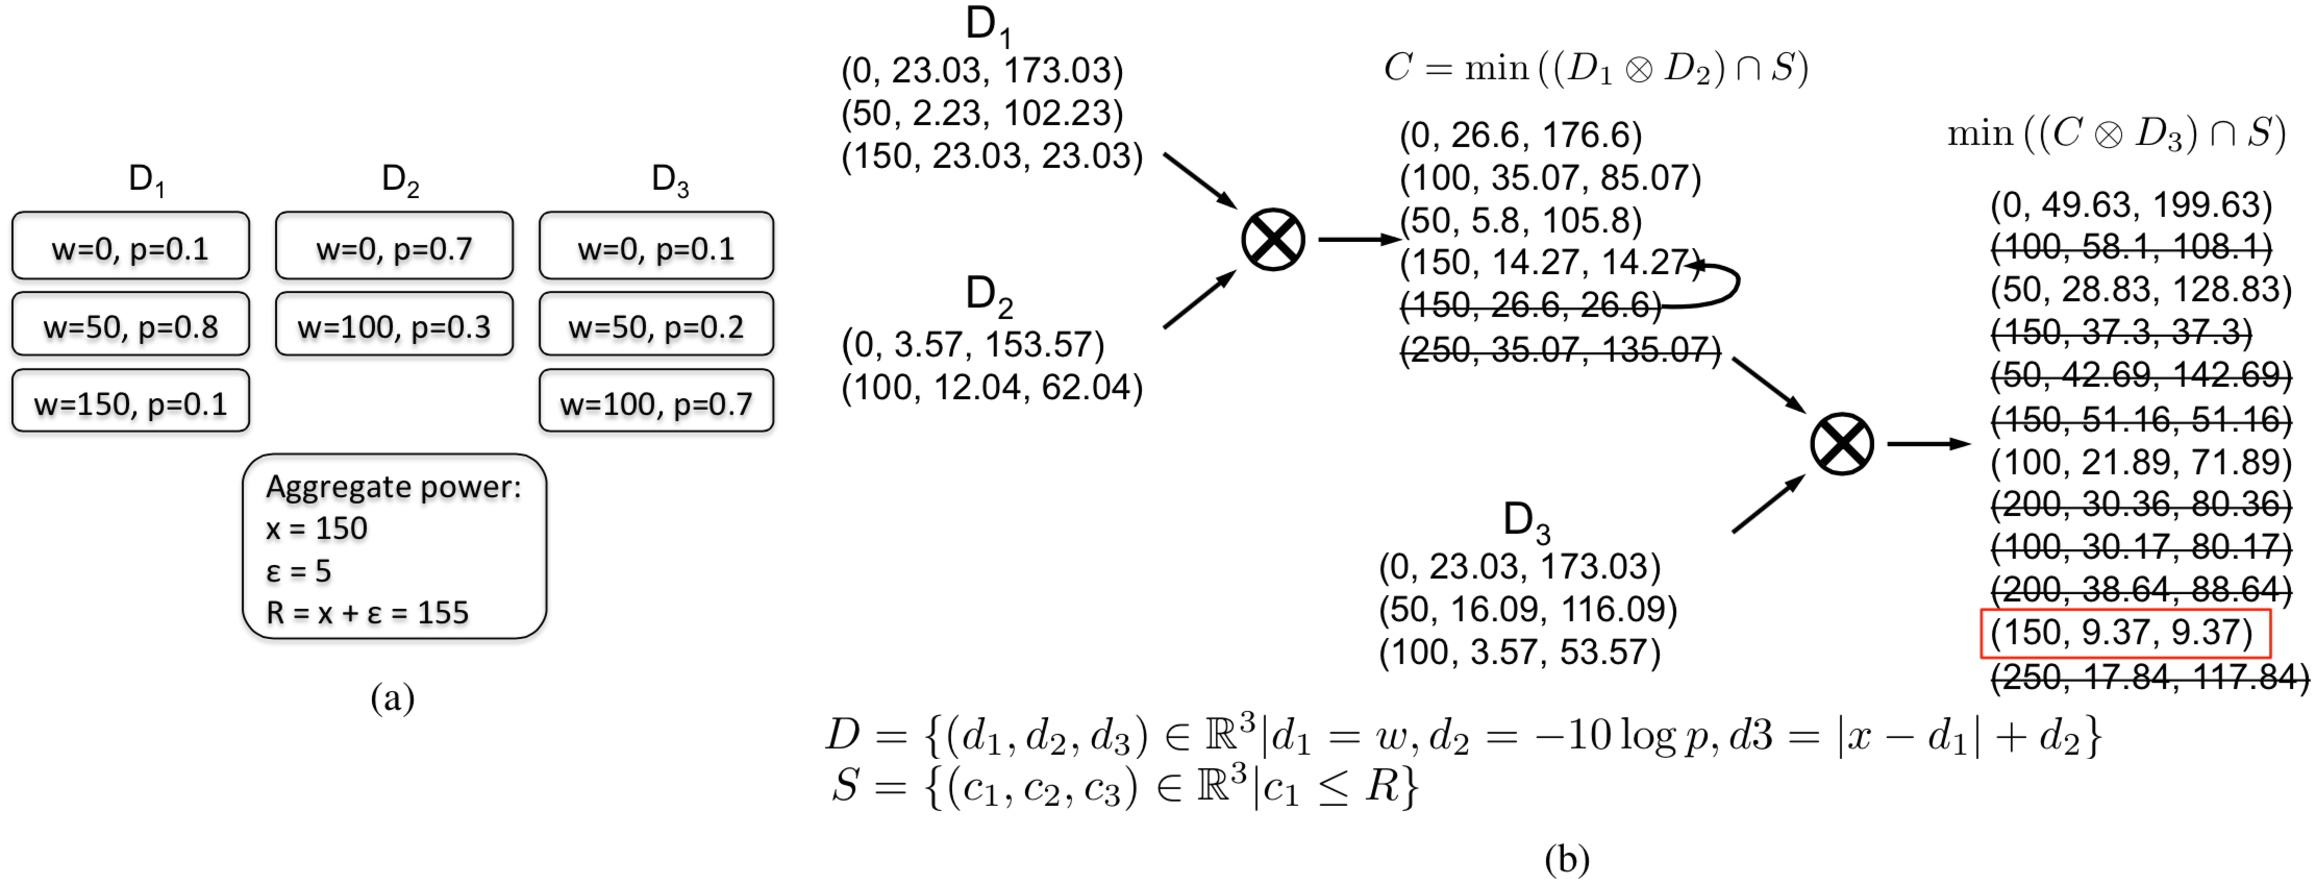
\includegraphics[width=1\textwidth]{./chapters/chapter4/images/CPHex.pdf} 
\caption{Running example of CPH. (a)~Three devices with corresponding power demand and probability of each state as well as the aggregate power consumption. (b)~Each device is represented as a set of tuples, each tuple corresponds to a state. At each iteration, a partial solution can be discarded if its first element (power consumption) exceeds the bound $R$ (rule~1), or its third element is greater than another solution while consuming larger or same power (rule~2). After all sets are combined, the tuple giving the smallest value of the third element is selected as the final solution.} 
\label{fig:SS2} 
\end{figure}

\begin{figure}[ht]
\centering
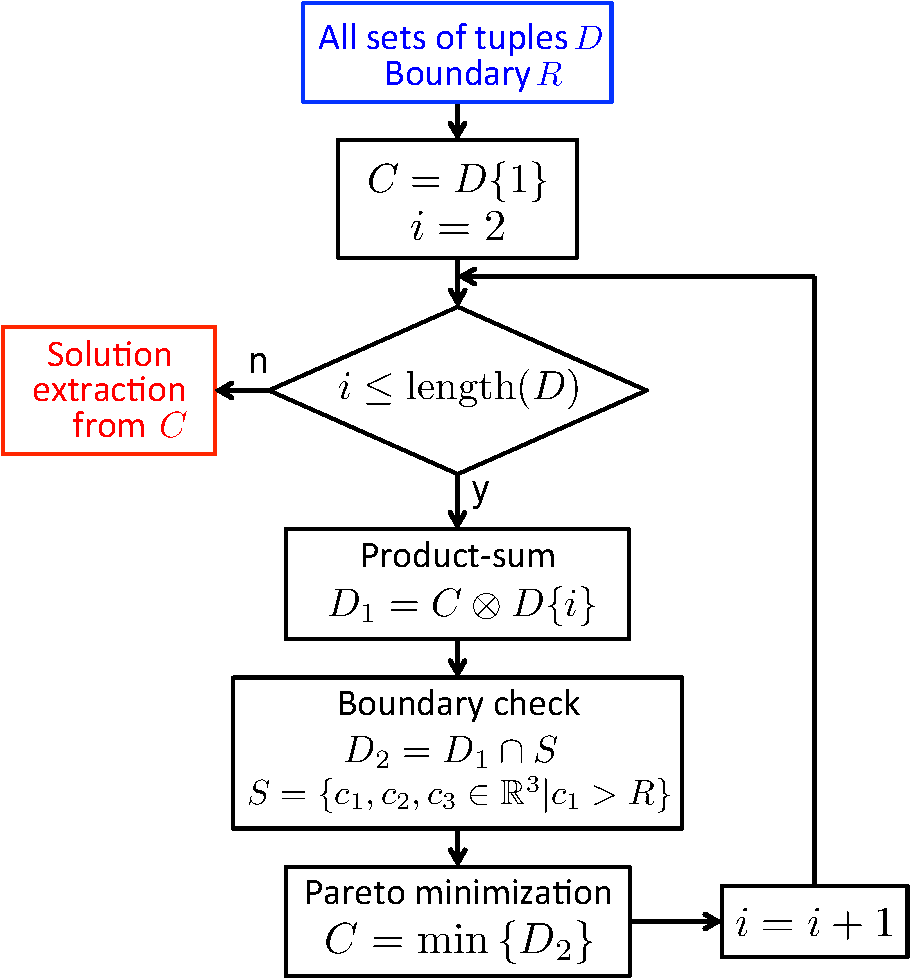
\includegraphics[width=0.55\textwidth]{./chapters/chapter4/images/CPHschema.pdf} 
\caption{CPH algorithm flowchart. All sets of tuples are saved in cell $D$. After the last iteration, the solution is extracted by selecting a tuple in $C$ with the least value of the third dimension.} 
\label{fig:SS2b} 
\end{figure}
In the second step, the sets of tuples are pairwise and iteratively combined by a so-called \textit{product-sum} operation~$\otimes$, which takes all possible combinations from two sets, sums their first and second elements per dimension and then calculates the third element by Eq.~\eqref{eqCPH1}. Some of the partial solutions will be discarded in the third step by two criteria. The first criterion to reject a tuple is that its power demand violates the bound $R$ (rule~1), denoted by the operation $(D_1 \otimes D_2)\cap S$, and the second one is that this tuple is dominated, i.e. it has a greater third value but the same or larger first value than another tuple (rule~2). This process is called \textit{Pareto minimization}~\cite{Shojaei13} and denoted by the operation $C=\min{((D_1 \otimes D_2)\cap S)}$, where $C$ contains the remaining solutions called \textit{Pareto points}. In the final step, after all sets are combined and the Pareto points are found, the point giving the smallest value in the third element is selected as the final solution. 

Figure~\ref{fig:SS2b} resumes the operation of CPH algorithm with
the procedure to combine two sets of tuples presented in Algorithm~\ref{algocph1} and the Pareto minimization illustrated in Algorithm~\ref{algocph2}. The notations $D_1 \preceq D_2$ and $D_1 \prec D_2$ mean that the tuple $D_1$ is dominated and strictly dominated, respectively, by $D_2$.

\begin{algorithm}
\caption{Combine two sets of tuples.} \label{algocph1}
\begin{algorithmic}[1]
\Function{AllComb}{$D_1,D_2,x$}
\State $l1 = \text{length}(D_1)$
\State $l2 = \text{length}(D_2)$
\For {$i=1,\ldots,l1$}
		 \For{$j=1,\ldots,l2$}
		    \State $D\{(i-1)l_1+j\}(1) = D_1\{i\}(1) + D_2\{j\}(1)$
		    \State $D\{(i-1)l_1+j\}(2) = D_1\{i\}(2) + D_2\{j\}(2)$
		    \State $D\{(i-1)l_1+j\}(3) = |D\{(i-1)l_1+j\}(1)-x|+D\{(i-1)l_1+j\}(2)$
		 \EndFor
\EndFor
\State output = $D$
\EndFunction
%\State \textbf{end function}
\end{algorithmic}
\end{algorithm}

\begin{algorithm}
\caption{Pareto minimization.} \label{algocph2}
\begin{algorithmic}[1]
\Function{ParetoMin}{$D,R$}
\State $l = \text{length}(D)$
\State $reject = \text{zeros}(l,1)$
\For {$i=1,\ldots,l$}
    \If {$D\{i\}(1)>R$}
	    \State $reject(i) = 1$
	\EndIf
\EndFor
\State $Ind = \text{find}(reject\neq 1)$
\State $D1 = D\{Ind\}$
\State $l1 = \text{length}(D1)$
\State $reject1 = \text{zeros}(l1,1)$
\For {$i=1,\ldots,l1-1$}
    \For {$j=i+1,\ldots,l1$}
        \If {$reject(j)\neq 1$ and $D1\{i\}\prec D1\{j\}$}
            \State $reject(i)=1$
        \ElsIf {$reject(j)\neq 1$ and $D1\{j\}\preceq D1\{i\}$}
            \State $reject(j)=1$
        \EndIf
    \EndFor
\EndFor
\State $Ind1 = \text{find}(reject1\neq 1)$
\State $D2 = D1\{Ind1\}$
\State output = $D2$
\EndFunction
%\State \textbf{end function}
\end{algorithmic}
\end{algorithm}


